\documentclass{article}[11pt]
\usepackage{minted}
\usepackage{graphicx}
\usepackage{float}
\usepackage{amsmath}

\title{6.047 Problem Set 5 Writeup}
\author{Matthew Feng}
\date{\today}

\begin{document}
\maketitle

\section{Positive selection in the human genome}
\subsection*{A.\quad Long haplotypes}
\subsubsection*{(a) Recent selection}
A haplotype block's length gives an indication of 
how recently that block appeared. Longer blocks
are more recent, while shorter blocks are more ancient,
since recombination has had time to decay the
haplotype block. In other words, an allele may rise
to high frequency rapidly enough that
long-range association with
nearby polymorphisms (i.e. the long-range haplotype)
will not have time to be eliminated by recombination.

\subsubsection*{(b) Individual polymorphisms}
With strong selection, the number of SNPs in the
candidate region will be quite large, and thus hard
to identify precisely which of those SNPs are the
polymorphisms under selection.

\subsubsection*{(c) XP-EHH Plots}
Recombinant frequencies (cM) are more preferable
because we are dealing with linkage disequilibria
and recombination; thus plotting based on
recombination frequencies allows us to have a
better scale of long haplotypes.

\begin{figure}[H]
    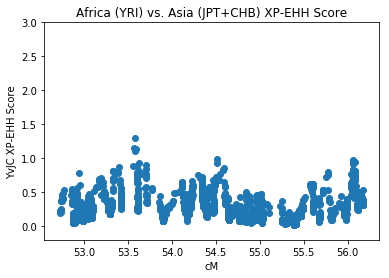
\includegraphics[width=0.8\textwidth]{problem1/yvjc.png}
\end{figure}

\begin{figure}[H]
    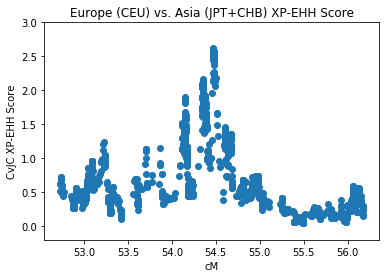
\includegraphics[width=0.8\textwidth]{problem1/cvjc.png}
\end{figure}

\begin{figure}[H]
    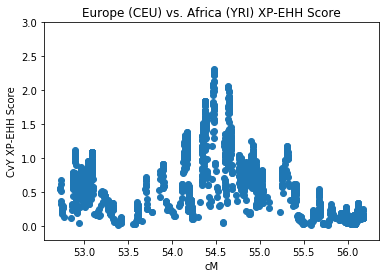
\includegraphics[width=0.8\textwidth]{problem1/cvy.png}
\end{figure}

\subsubsection*{(d) Subpopulation}
Subpopulation {\bf CEU (Europe)} seems to have the
strongest evidence for natural selection, as CvJC
and CvY XP-EHH scores both peak above 2.0 around 54.5cM,
but that peak does not appear in YvJC.

\subsubsection*{(e) XP-EHH $>$ 2.0}
\begin{minted}{python}
xpehh = pd.read_csv("./XPEHH.txt", sep="\t")
xpehh[(xpehh.iloc[:, 4] > 2.0) |
      (xpehh.iloc[:, 5] > 2.0) |
      (xpehh.iloc[:, 6] > 2.0)]
\end{minted}
79 SNPs (79 rows returned).

\subsection*{B.\quad Derived allele frequency}
\subsubsection*{(a) Ancestral alleles}
An error can occur when the chimpanzee base has mutated to the
same base of the derived human allele, or when the human allele
had a fixed mutation previously, and then recently a reversion
mutation. The probability of error is then

\[
    P_e = P_c(1 - P_c)(P_{same}) + (1 - P_c)(P_c)(P_{same}) \approx 0.6\%
\]

since $P_c \approx 1.23\% / 2$, and $P_{same}$, the probability
that the chimpanzee allele matches the human allele, is $0.5$.

\subsubsection*{(b) Derived allele frequencies}
\begin{figure}[H]
    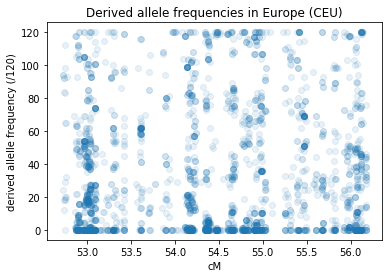
\includegraphics[width=0.8\textwidth]{problem1/derived_ceu.png}
\end{figure}

\subsubsection*{(c) Long haplotype and derived $>$ 0.6}
\begin{minted}{python}
derived = pd.read_csv("./Derived.txt", sep="\t")
hi_xpehh = (xpehh.iloc[:, 4] > 2.0) | 
           (xpehh.iloc[:, 5] > 2.0) |
           (xpehh.iloc[:, 6] > 2.0)
high_daf = derived.iloc[:, 5] > 0.6 * 120
derived[high_daf & hi_xpehh]
\end{minted}
22 SNPs.

\subsection*{C.\quad Population differentiation}
\subsubsection*{(a) $F_{ST}$ derivation}

\begin{align}
    H_T & = 2p(1 - p) \\
    H_S & = \dfrac{1}{2}(2(p + d)(1 - p - d) + 2(p - d)(1 - p + d))\\
        & = 2p - 2p^2 - 2d^2 \\
    \dfrac{H_T - H_S}{H_T} & = \dfrac{2p - 2p^2 - 2p + 2p^2 + 2d^2}{2p(1 - p)}\\
        & = \dfrac{d^2}{p(1-p)}.
\end{align}

Therefore, $F_{ST} = \dfrac{d^2}{p(1 - p)}$.

\subsubsection*{(b) $F_{ST}$ plots}
We can estimate $p$ by dividing the number of derived alleles by
the number of samples we have from the subpopulations; since
we have three subpopulations, we compute two $p$ values: one for
Europe and Africa (total $240 = 120 + 120$), and Europe and Asia
(total $300 = 120 + 180$). We can estimate $d$ by finding the
absolute difference in derived allele frequencies, dividing
by 2 (since there is both an addition and a subtraction),
and then normalizing over the number of samples ($240$ and $300$,
respectively).

\begin{figure}[H]
    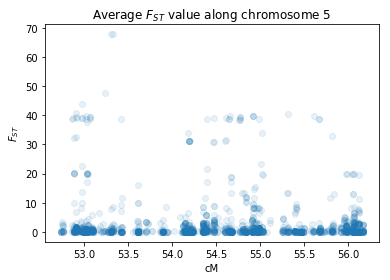
\includegraphics[width=0.8\textwidth]{problem1/fst.png}
\end{figure}

\subsubsection*{(c) Adding $F_{st} > 0.6$}
3 SNPs.

\subsection*{D.\quad Function}
\subsubsection*{(a) Conserved elements}
\begin{minted}{python}
s = 0
for x in xpehh.iloc[:, 2]:
    s += 1 if (len(cons[(cons.iloc[:, 1] <= x) &
                        (x <= cons.iloc[:, 2])])) > 0 else 0
\end{minted}

\noindent There are 105 SNPs that like within conserved elements.

\subsubsection*{(b) Final constraint}
There is only a single SNP that passes the above thresholds and lies within
a known or likely functional element.

\subsection*{E.\quad SNP}
SNP ID {\bf rs16891982}, part of the {\bf SLC45A2} gene which
is known to play a role in skin pigmentation.



\section{Maximum parsimony phylogeny}
\subsection*{A.\quad Tree costs}
\begin{figure}[H]
    \includegraphics[width=0.8\textwidth]{problem2/a.png}
\end{figure}

Cost of tree 1 (top left edge, bottom left, top right, bottom right, middle):
\begin{align*}
     &  0 + 2 + 0 + 0 + 1 + 2 \\
   + \ &  0 + 0 + 1 + 1 + 0 + 0 \\
   + \ &  0 + 0 + 0 + 0 + 0 + 0 \\
   + \ &  0 + 2 + 1 + 0 + 1 + 0 \\
   + \ &  1 + 1 + 0 + 0 + 2 + 0 \\
   = \ & \mathbf{15}
\end{align*}

Cost of tree 2 (top left edge, bottom left, top right, bottom right, middle):
\begin{align*}
     &  0 + 0 + 0 + 0 + 0 + 2 \\
   + \ &  1 + 2 + 0 + 0 + 2 + 0 \\
   + \ &  0 + 2 + 0 + 1 + 0 + 0 \\
   + \ &  1 + 0 + 0 + 0 + 2 + 0 \\
   + \ &  0 + 1 + 1 + 0 + 1 + 0 \\
   = \ & \mathbf{16}
\end{align*}

Cost of tree 3 (top left edge, bottom left, top right, bottom right, middle):
\begin{align*}
          &  1 + 1 + 0 + 0 + 2 + 2 \\
   + \ &  0 + 0 + 1 + 0 + 0 + 0 \\
   + \ &  0 + 1 + 0 + 0 + 0 + 0 \\
   + \ &  2 + 0 + 1 + 1 + 2 + 0 \\
   + \ &  0 + 2 + 0 + 0 + 1 + 0 \\
   = \ & \mathbf{17}
\end{align*}

Tree 1 is the minimum cost tree.

\subsection*{B.\quad UPGMA Clustering}
\begin{figure}[H]
    \includegraphics[width=0.8\textwidth]{problem2/b.png}
\end{figure}
    
No, it is not possible because the given distance matrix doesn't
satisfy the ultrametric constraint, where for any
three nodes $(a, b, c)$, $d_{ab} \le d_{bc} + d_{ac}$.
\end{document}